\begin{figure}[htbp]
\centering 
  \subfloat[Ratio over the volume occupied by the particles of each radius.]
  {
	  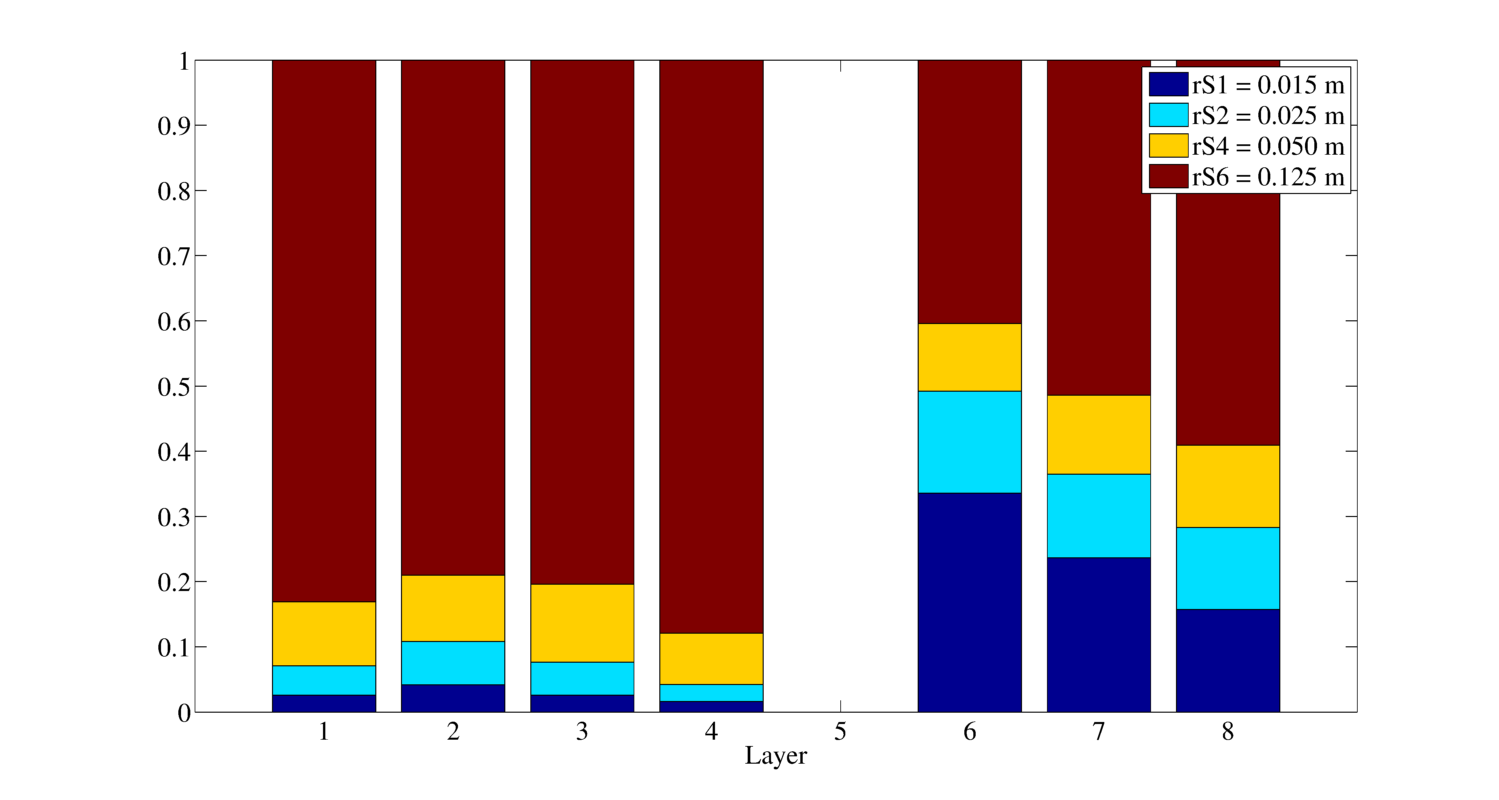
\includegraphics[width=.96\columnwidth]{images/121SinterBarPlot20151111150702}
	  \label{fig:121SinterBarPlot20151111150702}
  }
  \\
    \subfloat[Ratio over the number of the particles of each radius.]
    {
	  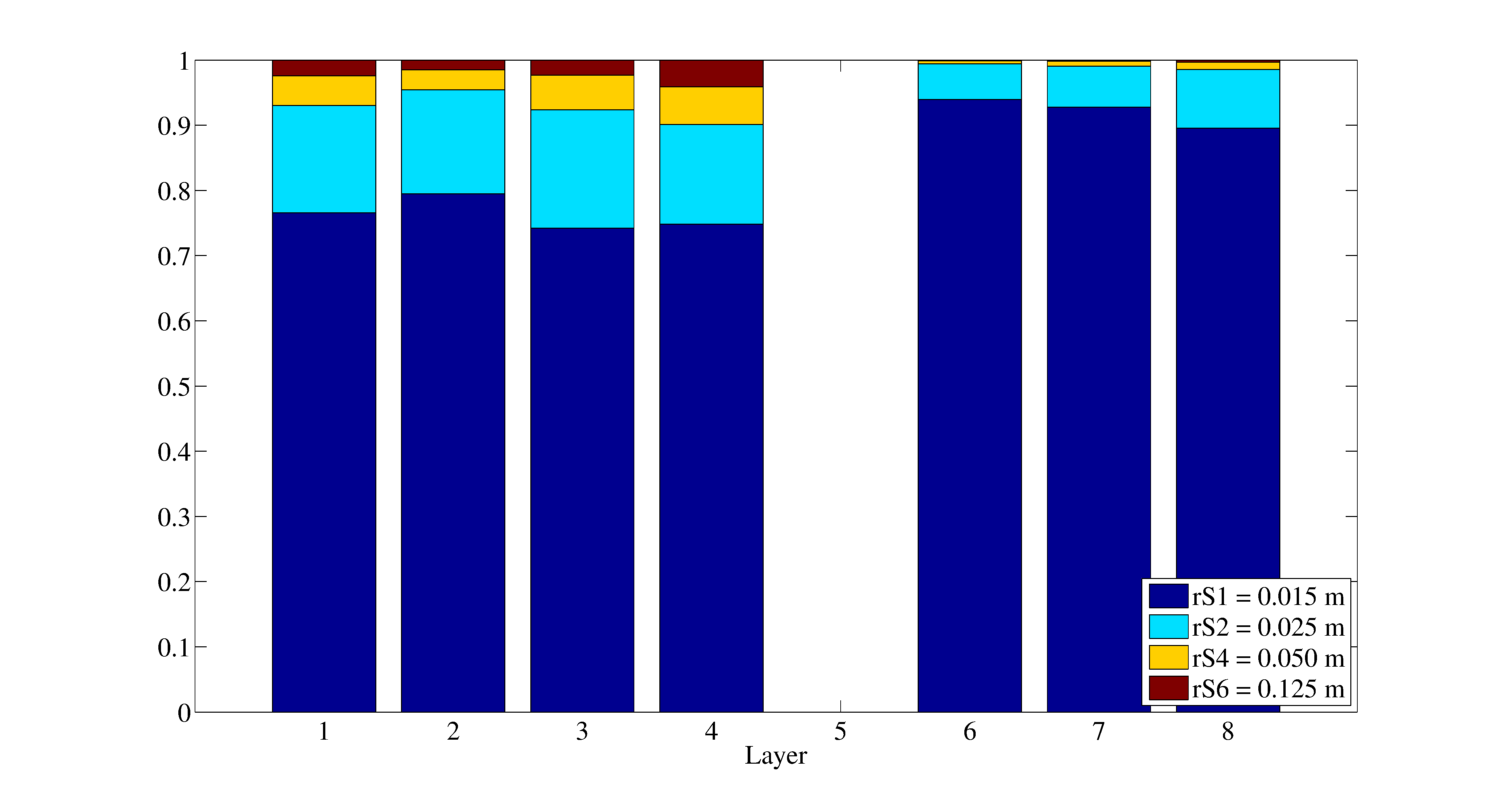
\includegraphics[width=.96\columnwidth]{images/122SinterBarPlot20151123180606}
	  \label{fig:122SinterBarPlot20151123180606}
  }
  \\
  \caption[Sinter bar plot]{Sinter bar plot. In the two plots we observe the
  higher likelihood of finding large particles in the bottom layers and small
  particles in the top layers.}
  \label{fig:066sinterbarplot}
\end{figure}